% \documentclass[journal]{IEEEtran}
\documentclass[12pt,journal,draftclsnofoot,onecolumn]{IEEEtran}
\IEEEoverridecommandlockouts

% remove colon after subsubsection, use spacing instead
\makeatletter
\renewcommand{\@IEEEsectpunct}{\quad}
\makeatother

\makeatletter
% add a small spacing *before* subsections
\let\origsubsubsection\subsubsection
\renewcommand\subsubsection{\@ifstar{\starsubsubsection}{\nostarsubsubsection}}

\newcommand\nostarsubsubsection[1]
{\subsubsectionprelude\origsubsubsection{#1}}

\newcommand\subsubsectionprelude{%
  \vspace{6pt}
}
\makeatother

% change default font to charter
% \usepackage{charter}
% \usepackage[bitstream-charter]{mathdesign}
% \usepackage{XCharter}
\usepackage{amsfonts}

% Fixing IEEEtran.cls bug with [english]{babel}
\makeatletter
\def\markboth#1#2{\def\leftmark{\@IEEEcompsoconly{\sffamily}\MakeUppercase{\protect#1}}%
\def\rightmark{\@IEEEcompsoconly{\sffamily}\MakeUppercase{\protect#2}}}
\makeatother

% \usepackage{t1enc}

\usepackage{listings}
\usepackage{multirow}
%\usepackage[utf8x]{inputenc}
\usepackage[english]{babel}
\selectlanguage{english}
\usepackage{color}
%\usepackage{caption}
\usepackage{cite}
\usepackage[pdftex]{graphicx}

% \usepackage{subfig}
\usepackage{subcaption}
\usepackage{amsmath}

\usepackage{mathtools}
\DeclarePairedDelimiter\ceil{\lceil}{\rceil}
\DeclarePairedDelimiter\floor{\lfloor}{\rfloor}

\usepackage{amsfonts}
\usepackage{array}
\usepackage{verbatim}
\usepackage{listings}
\usepackage{hyperref}
\usepackage{url}
\usepackage{enumerate}
\usepackage{multirow}

\usepackage{siunitx}
\usepackage{epsfig}
\usepackage{epstopdf}
\usepackage{multicol}% http://ctan.org/pkg/multicols
\usepackage[font=footnotesize]{caption}
% \usepackage[font=scriptsize]{subcaption}
% Tikz
\usepackage{tikz}
\usepackage{pgfplots}
\pgfplotsset{compat=newest}
\pgfplotsset{plot coordinates/math parser=false}
\newlength\fheight
\newlength\fwidth
\usetikzlibrary{patterns,decorations.pathreplacing,backgrounds,calc}
\definecolor{SchoolColor}{RGB}{0.71, 0, 0.106}%181,0,27} unipd red
\definecolor{chaptergrey}{rgb}{0.61, 0, 0.09} % dialed back a little
\definecolor{midgrey}{rgb}{0.4, 0.4, 0.4}
\definecolor{chaptergreen}{rgb}{0.09, 0.612, 0}
\definecolor{chapterpurple}{rgb}{0.522, 0, 0.612}
\definecolor{chapterlightgreen}{rgb}{0, 0.612, 0.522}

%\raggedbottom

% Pseudocode
\usepackage[ruled, vlined]{algorithm2e}

\SetKwRepeat{Do}{do}{while}
\SetKwProg{wp}{with probability }{ do}
\DontPrintSemicolon
% \usepackage{algorithm}
% \usepackage[noend]{algpseudocode}
% \renewcommand\algorithmicthen{}
% \renewcommand\algorithmicdo{}
\usepackage{lscape}

\addto\captionsenglish{\renewcommand{\figurename}{Fig.}}

\newcommand{\field}[1]{\mathbb{#1}}

\DeclareMathOperator*{\argmin}{arg\,min}
\DeclareMathOperator*{\argmax}{arg\,max}
\newcommand{\norm}[1]{\left\lVert#1\right\rVert}
\renewcommand{\arraystretch}{2}

\newcommand{\DP}[1]{\textbf{(DP: #1)}}
\newcommand{\el}[1]{\textr{(EL says: #1)}}
\newcommand{\fm}[1]{\texbf{(FM says: #1)}}

\usepackage{threeparttable}
%\usepackage[table,xcdraw]{xcolor}
\usepackage{tabularx}
\usepackage{multirow}
\usepackage{booktabs}
\newcommand{\tabitem}{~~\llap{\textbullet}~~}
\usepackage{array, blindtext}
\usepackage{wrapfig}
\usepackage{pdfpages}
\usepackage[acronym]{glossaries}

% use tikArchiviz images or eps
\newif\iftikz
\tikztrue

\graphicspath{{./figures/}}

\title{Heuristic optimization of Distributed Storage Network techniques}
\author{\IEEEauthorblockN{Federico Mason, Davide Peron, Enrico Lovisotto}\\
\small{{Department of Information Engineering, University of Padova -- Via Gradenigo, 6/b, 35131 Padova, Italy\\
Email: {\tt\{masonfed, perondav, lovisott\}@dei.unipd.it}\\}}
}

% Reduce the space below figs.
%\setlength{\belowcaptionskip}{-0.7cm}

\renewcommand{\equationautorefname}{Eq.}

%% Glossary
\newacronym{dsn}{DSN}{Distributed Storage Network}
\newacronym{edfc}{EDFC}{Exact Decentralized Fountain Codes}
\newacronym{adfc}{ADFC}{Approximate Decentralized Fountain Codes}
\newacronym{sa}{SA}{Simulated Annealing}
\newacronym{ga}{GA}{Genetic Algorithm}
\newacronym{jb}{JB}{Jumping Ball}
\newacronym{wsn}{WSN}{Wireless Sensor Network}
\newacronym{fp}{FP}{First Problem}
\newacronym{sp}{SP}{Second Problem}
\newacronym{of}{$f$}{Objective Function}
\newacronym{t}{T}{Temperature}
\newacronym{oc}{$x_o$}{Old Candidate}
\newacronym{nc}{$x_n$}{New Candidate}
\newacronym{sc}{$C_S$}{Step Coefficient}
\newacronym{ac}{$C_A$}{Acceptance Coefficient}
\newacronym{ap}{$P_A$}{Acceptance Probability}
\newacronym{ws}{$N_{WS}$}{Number of Worsening Steps}
\newacronym{wsmax}{$N_{WS}^{MAX}$}{ Maxiumum Number of Worsening Steps}
\newacronym{x}{x}{Candidate}
\newacronym{bestx}{$x_{best}$}{Best candidate}

\glsresetall
\begin{document}

\def\equationautorefname~#1\null{(#1)\null}
\setlength{\belowcaptionskip}{-0.2cm}

% reduce space after title
\makeatletter
\patchcmd{\@maketitle}
  {\addvspace{0.5\baselineskip}\egroup}
  {\addvspace{-1.2\baselineskip}\egroup}
  {}
  {}
\makeatother

\maketitle

\begin{abstract}
In some previous works about \gls{dsn}, two packet spreading algorithm are proposed, \gls{edfc} and \gls{adfc}.

Unfortunately the tuning procedure of their fundamental parameters, $x_d$ and $\nu$ respectively, was not thoroughly investigated.
We try then to explore these parameter spaces using heuristic optimization techniques, such as \emph{Simulated Annealing} and \emph{Genetic Algorithm}, to find suitable values for a broad range of network configurations.
\end{abstract}

\glsresetall
\section{Introduction} \label{sec:introduction}
In our setup, we consider a \gls{wsn} whose nodes are distributed over a known spatial region.
Some of them, called \textit{sensing nodes}, collect and deploy data from the environment (temperature, pressure, motion data, \ldots) while the others, called \textit{caching nodes}, simply store data coming from \textit{sensing nodes}.

In literature, a \gls{wsn} often has a central node, a powered sink connected to the internet.
Such special node receives all information collected by the network and provides it to the users.

owever, following our reference paper\cite{Lin2007}, we get rid of this assumption.
Users then must collect the data stored in the network visiting the geographical region where system is located.

In such a scenario, user visits only a certain number $h$ of nodes of the network.
To guarantee source packets decodability, \emph{Random Fountain Codes} are employed: $K$ source packets across $N$ total nodes are spread and combined such that, using any group of $K+\epsilon$ of them (with $\epsilon$ constant in $K$), the original information can be successfully retrieved with high probability.\cite{Luby}

The challenge here is to minimize the communication costs keeping a low and bounded failure probability.

Traditional but expensive \mbox{two-way} packet delivery is then discarded, in favor of \mbox{one-way} \emph{random walks}.
Packet routes are designed according to \emph{Metropolis algorithm} such that the number of packets reaching each node resembles the Robust Soliton distribution, whose optimal decoding properties are known.\cite{Luby}

In this paper, we are going to find the optimal $x_d$ and $\nu$ parameters for \gls{edfc} and \gls{adfc} respectively with three different heuristics and then test them with a network simulator, where further analysis is performed.

\smallbreak
This procedure is outlined in the following two sections.

In \autoref{sec:tech_approach} we describe \gls{adfc} and \gls{edfc} optimization problems and the heuristic algorithms employed to find the optimal points $x_d$ and $\nu$.

In \autoref{sec:results} we show how the optimal configurations provided by the heuristics behave in our network simulator, focusing on transmission costs and failure probability.

\section{Technical Approach}
\label{sec:tech_approach}
For a good packet spreading, \gls{edfc} and \gls{adfc} spreading algorithms require their parameters $x_d$ and $\nu$ to be carefully set before execution.
% rimandiamo al paper per una descrizione migliore: qua ne parliamo solo un attimo per far capire cosa abbiamo fatto

\smallbreak
According to \gls{edfc} algorithm, a node of chosen degree $d$, realization of the reference \emph{Robust Soliton Distribution}, should receive at the end of the spreading phase $x_d \, d$ packets, where $x_d$ is called \emph{redundancy coefficient}.

The following optimization problem aims to reduce at the minimum the transmission cost introduced by this approach, ensuring at the same time an upper bound to the failure probability $\delta$.\cite{Lin2007}

\begin{equation}
	\label{eq:fp}
	\tag{FP}
	\begin{split}
		minimize \quad & \sum_{d=1}^K x_d d \mu (d) \\
		given \quad & \begin{dcases}
			Pr(Y<d|X=d) \leq \delta \\
			x_d \geq 1 \text{ ~for~ } d = 1, \, \ldots, \, K
		\end{dcases} \\
		where \quad & \begin{dcases}
			Y \sim Bin(K, p) \\
			p = 1 - \left( 1 - \frac{x_d \, d}{NE} \right) ^ {NE / K} \\
			E = \sum_{i = 1}^{K} \mu(d) \, x(d) d
		\end{dcases} \\
	\end{split}
\end{equation}

\bigbreak

\gls{adfc} optimization problem tries instead to find a suitable probability distribution $\nu$ for nodes degree such that, after package spread, the resulting degree distribution $\nu^\prime$ across the network is as close as possible to the reference distribution.

\begin{equation}
	\label{eq:sp}
	\tag{SP}
	\begin{split}
		minimize & \quad \sum_{i=1}^{K}(\nu'(i)-\mu(i))^2 \\
		given & \quad \begin{dcases}
			\sum_{i=1}^K \nu(i) = 1 \\
			\nu(i) \geq 0 \text{~~for~~} i=1,...,K
		\end{dcases} \\
		where & \quad
		\begin{dcases}
			v^\prime(i) = \sum_{d=1}^K \nu(d) \,\binom{K}{i} \, p^i \, (1-p)^{K-i} \\
			p = 1 - \left(1 -\frac{d}{N E}\right)^{{N E} / {K}} \\
			E = \sum_{i = 1}^{K} \nu(d) d
		\end{dcases}
	\end{split}
\end{equation} \vspace{0cm}

We can notice immediately that \autoref{eq:fp} and \autoref{eq:sp} are not solvable with \emph{convex optimization} techniques, as they don't minimize convex objective functions over convex sets.

Since traditional tools (such as \emph{simplex} or \emph{gradient descent}) cannot be applied, we chose some heuristic approaches, whose convergence to the optimum is not guaranteed in polynomial time, but whose effectiveness has been proven in many fields.\cite{Edelkamp2010}.

\subsection{Perturbation strategies} \label{sec:perturbations}
In order to explore problem solution space effectively, each heuristic technique requires a primitive function called \emph{perturbation}.
Given a valid parameter configuration, this routine should provide a new point \emph{nearby} the current one that satisfies problem constraints.
Such candidate solution is then accepted or rejected given its objective function value, according to the various research algorithms.

\smallbreak
Since the two considered problems are very different with respect to their constraints, we developed two different strategies, whose pseudocode is available in \autoref{algo:perturb_edfc} and \autoref{algo:perturb_adfc} respectively.

Exploiting this primitive, all heuristic search tecniques detailed later in this paper refer to a general problem, abstracting from \gls{adfc} and \gls{edfc} peculiarities.

\clearpage
\begin{algorithm}[htp]
\caption{\gls{edfc} perturbation} \label{algo:perturb_edfc}
	\KwIn{Primitive \emph{respect constraints} for \gls{edfc}, $\vec{x}_{old}$}
	\KwOut{vector of redundancy coefficients $\vec{x}_{new}$}

	\Repeat{$\vec{x}_{new}$ \emph{respects constraints}} {
		$\vec{x}_{new}$ $\gets$ copy($\vec{x}_{old}$) \\
		pick an integer $d \sim \mathcal{U}([1, K])$ \\
		pick a real number $\Delta \sim \mathcal{U}([-2T, T])$ \\
		$\vec{x}_{new}$[d] = $\vec{x}_{new}$[d] + $\Delta$
	}
	\Return{$\vec{x}_{new}$}
\end{algorithm}

\begin{algorithm}[htp]
\caption{\gls{adfc} perturbation} \label{algo:perturb_adfc}
	\KwIn{Primitive \emph{respect constraints} for \gls{adfc}, vector of probabilities $\nu_{old}$}
	\KwOut{valid probability distribution}
	\Repeat{$\nu_{new}$ \emph{respects constraints}} {
		$\nu_{new} \gets$ copy($\nu_{old}$) \\
		\Repeat{$\nu_{new}(d_1) \ne 0$}{
			pick $d_1 \sim \mathcal{U}([1, K])$
		}

		\Repeat{$d_1 \neq d_2 ~\land~ v_{new}(d_2) \neq 0$}{
			pick $d_2 \sim \mathcal{U}([1, K])$ \\
		}

		$ h \gets \min\{\nu_{new}(d_1), \nu_{new}(d_2)\} $ \\
		pick a real number $\Delta \sim \mathcal{U}([0, h])$ \\

		$\nu_{new}(d_1) \gets \nu_{new}(d_1) - \Delta$ \\
		$\nu_{new}(d_2) \gets \nu_{new}(d_2) + \Delta$ \\
	}
	\Return{$\nu_{new}$}
\end{algorithm}

\clearpage
\subsection{Simulated Annealing}
The first algorithm we implement is known as \gls{sa}.
It is a probabilistic technique that takes ispiration from annealing in metallurgy, a process that aims to reduce materials defects.
In this physical process a piece of metal is warmed at high temperatures and then slowly cooled. In this way it is possible to achieve the molecular equilibrium inside the material itself.

In \gls{sa}, we treat \gls{of} as the internal energy of the material.
As in the physical process we want to reduce the function energy and slowly bring it to a stable value. In other words we want first to cross widely the function domain and then to concentrate in the points with higher probability to be the absolute minimum of \gls{of}.

\gls{sa} behaviour is dependent on a parameter called \gls{t}: relevant for the search are \gls{sc} and \gls{ac}, the number of points to inspect for given \gls{t} and the probability $P_A$ of accepting a point worse than the current, respectively. At the beginning \gls{t} is initialized at a sufficient high value and then it is reduced at each algorithm step.

The process starts at a random configuration $\vec{\gamma} = [\gamma_1, \ldots, \gamma_K]$ respecting problem constraints.
Then, each new point $\vec{\gamma}_{new}$ is found \emph{perturbing} previous vector $\vec{\gamma}$, as described in \autoref{sec:perturbations} for \gls{adfc} and \gls{edfc} algorithms.

The proposed solution is kept or rejected according to the \gls{ap}, whose expression is the following.
\begin{equation*} \label{accept_prob}
	P_A(\Delta, T) = \begin{cases}
		1 & \Delta < 0 \\
		\mathrm{e}^{ - C_A \, \Delta / T }
		& \Delta \geq 0
	\end{cases}
	\quad \quad \text{where} \quad \Delta = f(\gamma_{new})-f (\gamma)
\end{equation*}

The best point among all the explored ones is kept across the path and it is returned at the end of the computation.
A pseudocode for this procedure can be found in \autoref{algo:SA}.

\begin{algorithm}
	\KwIn{Objective function $f$ and constraints,
		Initial Temperature,
		Maximum number of steps,
		Steps Coefficient,
		Acceptance Coefficient,
		Perturb function}
\KwOut{Optimal solution}
\caption{Simulated Annealing} \label{algo:SA}
$T \gets$ Initial Temperature \\
$\gamma \gets$ Random valid point \\
$\gamma_{best} \gets \gamma$ \\
$C_A \gets$ Acceptance coefficient \\
$N_S \gets 0$ \\
$N_S^{MAX} \gets $ Maximum number of steps \\

\While{$N_S < N_S^{MAX}$} {
	$C_S \gets$ Steps coefficient ($T$) \\
	\For{$i = 1$ to $C_S$} {
		\vspace{1mm}
		$\gamma_{new} \gets$ Perturb$(\gamma)$\\
		$\Delta \gets f(\gamma_{new})-f(\gamma)$ \\
		\wp{$P_A(\Delta, T)$}{
			\vspace{1mm}
			$\gamma \gets \gamma_{new}$\\
			\If{$f(\gamma)<f(\gamma_{best})$}{
				\vspace{1mm}
				$\gamma_{best} \gets \gamma$\\
			}
		}
		Increment $N_S$
		update $C_S$\\
	}
}
\Return{$\gamma_{best}$}
\end{algorithm}

\subsection{Jumping Ball}

Our second search algorithm is a variation of \gls{sa}, called \gls{jb}, designed and implemented by our group.

Its approach rose from the observation that if the cooling phase of \gls{sa} takes to a sub-optimal region of the solution space there is no way to leave it for a better one.

So, we develop the heuristic of \emph{jumps}, whose aim is to overcome this issue. If the best solution available is not improved for a certain number $N_{WS}^{MAX}$ of small steps, as done in \gls{sa}, a \emph{jump} is performed perturbating lots of components all at once of a big extent.

$N_{WS}^{MAX}$ has to be initialized properly: a value too low would lead the algorithm to jump indefinitely without ever stabilizing in a single area, but a value too high would make jumps impossible, making pointless this variation.
A proper value instead enhances the exploration space of the \gls{sa} algorithm, leading to hopefully better results in our variant \gls{jb}.

The pseudocode for \gls{jb} is the same as \gls{sa}, the different \emph{Perturb} function is described in \autoref{algo:JB_neigh}.

\begin{algorithm}
	\caption{Jumping Ball \emph{Perturb}}\label{algo:JB_neigh}
	\KwIn{Problem constraints and objective function $f$, $\gamma$, $N_{WS}^{MAX}$, current number of worsening steps $N_{WS}$}
	\KwOut{$\gamma_{new}$}
	\Repeat{$\gamma_{new}$ \emph{respects constraints}} {
		$\gamma_{new} \gets \gamma$ \\
		\If { $N_{WS} > N_{WS}^{MAX}$ } {
			\Repeat{$\gamma_{new}$ \emph{respects constraints}} {
				Perturb a random number of components of $\gamma_{new}$
			}
			$N_{WS}$ = 0
		}
		\Else {
			Perturb just one component of $\gamma_{new}$ in $[1, \,K]$
		}
	}
	\If { $f(\gamma_{new}) > f(\gamma_{best})$  } {
		Increment $N_{WS}$
	}
	\Return $\gamma_{new}$
\end{algorithm}

\clearpage
\subsection{Genetic Algorithm}

Our third technique is an implementation of \gls{ga}, framework that takes randomly an initial set of solutions for the problem and tries to evolve this \emph{population} of points toward better values.

According to the biological interpretation, each candidate solution, in our case a multi-dimensional vector, is an \emph{individual}.
Then each of its components is called \emph{chromosome} or \emph{genotype} and the subsequent iterations to explore the solution space \emph{generations}.

In each step of the algorithm the worst performing individuals of the current population are discarded and replaced by \emph{mutations} of the best individuals, that survives to the next round.

In this work we have decided to keep the 25\% best individuals of the current generation for the next one and obtain the remaining three quarters perturbing one, two and three components of the previous ones respectively. Perturbations are performed as described earlier in \autoref{sec:perturbations}, depending on the considered problem.

Our \gls{ga} can be tuned with the following parameters.
\begin{description}
	\item[\textbf{Survival Rate}] \hfill \\
	The fraction of population that is used to create the next generation. A survival rate too high forces the algorihm to discard worse, but potentially interesting paths in favour of the current best, while a value too low reduces the progress across generations.
	\item[\textbf{Max Generations}] \hfill \\
	Number of generations, the iterations of the algorithm. Note that exploration time is linear in this parameter.
	\item[\textbf{Population size}] \hfill \\
	Number of individual in a population. Increasing this parameter enhances performances but increase slightly the memory load and to a greater extent computation time.
\end{description}


\begin{algorithm}
	\KwIn{
		Objective function and constraints,
		survival rate,
		max generations,
		population size}
	\KwOut{Optimal solution}
	population $\gets$ get initial population(population size) \\
	$\alpha \gets$ survival rate \\
	$n_{gen} \gets 0$ \\
	$n_{gen}^{MAX} \gets$ max generations \\
	\While{$n_{gen} < n_{gen}^{MAX}$}{
		\vspace{1mm}
		sort population by objective function\\
		\For{$i=1$ to $\floor{ 1 / \alpha}$}{
			\For{\emph{portion} $=1$ to $\alpha \, ($\emph{population size}$)$} {
				current good point $\gets$ population[i] \\
				population[i + $\alpha ($population size$)$ portion] $\gets$ perturb(current good point) \\
			}
		}
		Increment $n_{gen}$ \\
	}
	\Return{\emph{population[0]}}
	\caption{Genetic Algorithm}\label{algo:GA}
\end{algorithm}

\clearpage
\section{Results} \label{sec:results}
In this section we compare the proposed spreading algorithms, \gls{edfc} and \gls{adfc}, in different scenarios, spanning from smaller neworks of hundreds of elements to bigger ones with thousands of nodes.
We followed our reference papers \cite{Lin2007} \cite{Aly2008} with respect to degree distribution parameters, as well as system fault tolerance, to obtain consistent results.

All network configurations details, as well as the main numerical results, can be retrieved in \autoref{tab:results} and following plots.

\subsection{Optimization}
First of all, we solved the two optimization problems for the various parameter settings using the three heuristics described in \autoref{sec:tech_approach}.

Along each network parameters, \autoref{tab:results} provides overhead coefficients $g_1$ and $g_2$ of problems \autoref{eq:fp} and \autoref{eq:sp} respectively, for each optimal solution for $\vec{x}$ and $\nu$.\cite{Lin2007}

\begin{equation*}
	\openup 1\jot % increase spacing between lines
	\begin{split}
		g_1(\vec{x}) &= \frac{\sum_{d=1}^K x_d d \mu (d)}{\sum_{d=1}^K d \mu (d)} \\
		g_2(\nu) &= \frac{\sum_{d=1}^K \nu(d) \, d \mu (d)}{\sum_{d=1}^K d \mu (d)}
	\end{split}
\end{equation*} \vspace{0cm}

Note that some results of \gls{sa} and \gls{jb} for configuration \emph{a)} are omitted in \autoref{tab:results}, because solutions found in the \gls{adfc} framework were highly sub-optimal with respect to overhead parameter $g_2$.

Moreover, \gls{ga} is the clear  winner in \gls{adfc} context, where it is more robust than the others and provides always a good result.
We think dynamic heuristic of \gls{ga} is more suitable to explore this complex solution space, while simpler approach employed in the others tends to stay always close to the starting point.

This observation is confirmed by our work, since in the simpler situation of \gls{edfc} the optimal points provided by the three heuristics are very close respect to cost coefficient $g_1$.

\smallbreak
Regarding computation time of \gls{edfc} optimization, \gls{jb} was slightly faster to reach convergence than \gls{sa}, thanks to our jumping heuristic that allowed to a more aggressive strategy at the beginning, in highly suboptimal regions of solutions space.
Both were still slower though than \gls{ga} in all configurations, except big network \emph{a)}, but by a small margin.

The second problem, \gls{adfc} has been much more difficult to deal with, because of the computational complexity of its objective function: while in \gls{edfc} the scalar product in $\mathbb{R}^K$ requires time $O(K)$, the double sum of \autoref{eq:sp} requires time $O(K^2)$.

This was unfeasible for big network configurations, where heuristic search process took too long to obtain a solution in reasonable time, so we decided to speed up the process at the cost of an approximated value for the objective function.

In paper\cite{Lin2007}, the proposal was to drop the contribute of coefficients after index $K/R$, since reference Robust Soliton distribution probability is considered irrelevant in that region.

We discard this hypothesis, proposing an adaptive strategy:
since the proposed perturbation strategy for \gls{adfc} modifies only two components of the solution array at a time, we decided to update only the correspoding terms of the sum in \autoref{eq:sp}.
This approach neglects the other $K-2$ terms of the sum, supposing they are almost unchanged.
This hypothesis has proven correct in practice, where error with respect to correct computation is negligible, but computational complexity is reduced from $O(K^2)$ to $O(K)$.

As can be seen in \autoref{fig:progress-adfc}, the best solver for \gls{adfc} problem is clearly \gls{ga}, because \gls{jb} and \gls{sa} solutions were highly suboptimal in some contexts, e.g. \emph{a)}, or the path to reach them was rough, far from the optimal region of the solution space.
Again, we think that \gls{ga} heuristic was more powerful and fit to the problem.

\subsection{Simulation}
\gls{adfc} and \gls{edfc} were then run in our network simulator, to test all degree distributions found at optimization step.
We supposed a fully reliable channel and implemented then a network layer simulator: this was done to assess the viability of the coding scheme in a general context, regardless of physical and medium access protocol peculiarities.

As customary in literature, wireless sensors were modeled as a set of points uniformly spread in a reference area where each one could communicate only with all near nodes, according to a distance parameter.

\subsubsection{Transmission cost}
For each run of our simulation, we report in \autoref{tab:results} relevant spreading quantities, in particular average length $L_{rw}$ of random walks taken by each packet, number of packets $n_{pkt}$ spread across the network and total number $n_{tx}$ of packet transmissions.
We focused on these few scores to highlight the total cost of each algorithm with the solutions provided by our heuristics.

\smallbreak
With respect to \gls{edfc} solutions, we noticed that our three heuristics find similar points, except in network \emph{a)}, where \gls{ga} is the best one by a significant margin.

\gls{adfc} solutions, instead, provided the lowest transmission cost, expecially
for \gls{ga}, that is the clear winner across all network setups and spreading tecniques.

\smallbreak
Our best scores, with respect to overhead parameters $g_1$ and $g_2$, on configuration \emph{a)} are very close to the ones obtained in our reference paper\cite{Lin2007}, confirming the results obtained by its research group.

\subsubsection{Successful decoding probability}
Transmission cost, however, is only one side of the coin: in order to be effective, packets have to be recovered in reasonable time by the user.

For the various network configurations labeled in \autoref{tab:results}, we then tested how average successful decoding probability changes with different decoding ratios $\eta$, defined as the number of packets collected by the user normalized by $K$.

As can be see in \autoref{fig:eta_vs_prob_adfc_only}, \gls{adfc} solutions provided by \gls{sa} and \gls{jb} could not provide a working network in almost all conditions proposed, while \gls{ga} found suitable configurations, that are then compared to \gls{edfc} one in \autoref{fig:eta_vs_prob_reliable_ones}.

Here it is clear that the reduce transmission cost provided by \gls{adfc} has a price: in some configurations, especially \emph{a)}, \emph{e)} and \emph{g)},  decoding probability is significantly worse than the others, albeit reducing the transmission cost up to three order of magnitudes.

Setting \emph{f)} is a prime example of this observation, where a similar success probability is obtained, with a fraction of the transmission cost.

\clearpage
\begin{table}[htp]
	\centering
	\renewcommand{\arraystretch}{0.9}
\begin{tabular}{c c c c c c c c c c c c} \toprule
& $K$ & $N$ & $c$ & $\delta$ & Problem & Solver & $g_1$ & $g_2$ & $L_{rw}$ & $n_{pkt}$ & $n_{tx}$ \\
\cmidrule{2-12}
\multirow{6}{*}{a)} & \multirow{6}{*}{1\,000} & \multirow{6}{*}{2\,000} & \multirow{6}{*}{0.01} & \multirow{6}{*}{0.05}
  & \multirow{3}{*}{EDFC}
     & GA & 1.72328 &  & 3589 & 25000 & $8.97 \times 10^{7}$ \\
&&&&&& SA & 1.89216 &  & 3940.11 & 28000 & $1.10 \times 10^{8}$ \\
&&&&&& JB & 1.89966 &  & 3956.04 & 28000 & $1.11 \times 10^{8}$ \\
 &&&&& \multirow{3}{*}{ADFC}
     & GA &  & 0.390452 & 1986.83 & 5000 & $9.93 \times 10^{6}$ \\
&&&&&& SA &  & 64.0368 &  &  & \\
&&&&&& JB &  & 67.6922 &  &  & \\
\cmidrule{2-12}
\multirow{6}{*}{b)} & \multirow{6}{*}{10} & \multirow{6}{*}{100} & \multirow{6}{*}{0.1} & \multirow{6}{*}{0.5}
  & \multirow{3}{*}{EDFC}
     & GA & 2.63602 &  & 263.916 & 770 & $2.03 \times 10^{5}$ \\
&&&&&& SA & 2.64062 &  & 267.839 & 770 & $2.06 \times 10^{5}$ \\
&&&&&& JB & 2.63926 &  & 267.401 & 770 & $2.06 \times 10^{5}$ \\
&&&&& \multirow{3}{*}{ADFC}
     & GA &  & 0.906249 & 93.3731 & 260 & $2.43 \times 10^{4}$ \\
&&&&&& SA &  & 0.682834 & 95.99 & 200 & $1.92 \times 10^{4}$ \\
&&&&&& JB &  & 1.31408 & 100.247 & 380 & $3.81 \times 10^{4}$ \\
\cmidrule{2-12}
\multirow{6}{*}{c)} & \multirow{6}{*}{20} & \multirow{6}{*}{100} & \multirow{6}{*}{0.1} & \multirow{6}{*}{0.5}
  & \multirow{3}{*}{EDFC}
     & GA & 2.35404 &  & 227.518 & 840 & $1.91 \times 10^{5}$ \\
&&&&&& SA & 2.36511 &  & 228.225 & 840 & $1.92 \times 10^{5}$ \\
&&&&&& JB & 2.36682 &  & 228.225 & 840 & $1.92 \times 10^{5}$ \\
&&&&& \multirow{3}{*}{ADFC}
     & GA &  & 0.750817 & 97.1769 & 260 & $2.53 \times 10^{4}$ \\
&&&&&& SA &  & 4.47709 & 99.0288 & 1600 & $1.58 \times 10^{5}$ \\
&&&&&& JB &  & 2.69659 & 93.05 & 960 & $8.93 \times 10^{4}$ \\
\cmidrule{2-12}
\multirow{6}{*}{d)} & \multirow{6}{*}{20} & \multirow{6}{*}{200} & \multirow{6}{*}{0.1} & \multirow{6}{*}{0.5}
  & \multirow{3}{*}{EDFC}
     & GA & 2.36865 &  & 509.038 & 1700 & $8.65 \times 10^{5}$ \\
&&&&&& SA & 2.37957 &  & 509.682 & 1700 & $8.66 \times 10^{5}$ \\
&&&&&& JB & 2.3792 &  & 509.514 & 1700 & $8.66 \times 10^{5}$ \\
  &&&&& \multirow{3}{*}{ADFC}
     & GA &  & 0.75314 & 189.748 & 540 & $1.02 \times 10^{5}$ \\
&&&&&& SA &  & 4.47709 & 202.238 & 3220 & $6.51 \times 10^{5}$ \\
&&&&&& JB &  & 2.69659 & 212.192 & 1940 & $4.12 \times 10^{5}$ \\
\cmidrule{2-12}
\multirow{6}{*}{e)} & \multirow{6}{*}{40} & \multirow{6}{*}{200} & \multirow{6}{*}{0.1} & \multirow{6}{*}{0.5}
  & \multirow{3}{*}{EDFC}
     & GA & 2.25899 &  & 516.791 & 1920 & $9.92 \times 10^{5}$ \\
&&&&&& SA & 2.17902 &  & 492.427 & 1840 & $9.06 \times 10^{5}$ \\
&&&&&& JB & 2.17781 &  & 492.427 & 1840 & $9.06 \times 10^{5}$ \\
  &&&&& \multirow{3}{*}{ADFC}
     & GA &  & 0.634248 & 189.162 & 520 & $9.84 \times 10^{4}$ \\
&&&&&& SA &  & 8.81251 & 197.003 & 7520 & $1.48 \times 10^{6}$ \\
&&&&&& JB &  & 4.42144 & 211.529 & 3760 & $7.95 \times 10^{5}$ \\
\cmidrule{2-12}
\multirow{6}{*}{f)} & \multirow{6}{*}{50} & \multirow{6}{*}{500} & \multirow{6}{*}{0.01} & \multirow{6}{*}{0.5}
  & \multirow{3}{*}{EDFC}
     & GA & 2.13626 &  & 2372.87 & 6600 & $1.57 \times 10^{7}$ \\
&&&&&& SA & 2.10669 &  & 2334.43 & 6500 & $1.52 \times 10^{7}$ \\
&&&&&& JB & 2.11034 &  & 2336.95 & 6500 & $1.52 \times 10^{7}$ \\
  &&&&& \multirow{3}{*}{ADFC}
     & GA &  & 0.483978 & 507.091 & 1500 & $7.61 \times 10^{5}$ \\
&&&&&& SA &  & 0.79639 & 519.944 & 2450 & $1.27 \times 10^{6}$ \\
&&&&&& JB &  & 3.70096 & 519.206 & 11450 & $5.94 \times 10^{6}$ \\
\cmidrule{2-12}
\multirow{6}{*}{g)} & \multirow{6}{*}{100} & \multirow{6}{*}{1\,000} & \multirow{6}{*}{0.1} & \multirow{6}{*}{0.5}
  & \multirow{3}{*}{EDFC}
     & GA & 1.96512 &  & 3757.41 & 14200 & $5.34 \times 10^{7}$ \\
&&&&&& SA & 1.97178 &  & 3768.47 & 14300 & $5.39 \times 10^{7}$ \\
&&&&&& JB & 1.96771 &  & 3761.16 & 14200 & $5.34 \times 10^{7}$ \\
  &&&&& \multirow{3}{*}{ADFC}
     & GA &  & 0.410634 & 1032.85 & 2900 & $3.00 \times 10^{6}$ \\
&&&&&& SA &  & 4.25821 & 1049.11 & 30900 & $3.24 \times 10^{7}$ \\
&&&&&& JB &  & 6.96241 & 1031.95 & 50500 & $5.21 \times 10^{7}$ \\
\bottomrule
\end{tabular}

%%% Local Variables:
%%% mode: latex
%%% TeX-master: "dystoNet"
%%% End:

	\caption{Complete results for all network configurations considered, marked with letters.}
	\label{tab:results}
\end{table}

\begin{figure}[htp]
	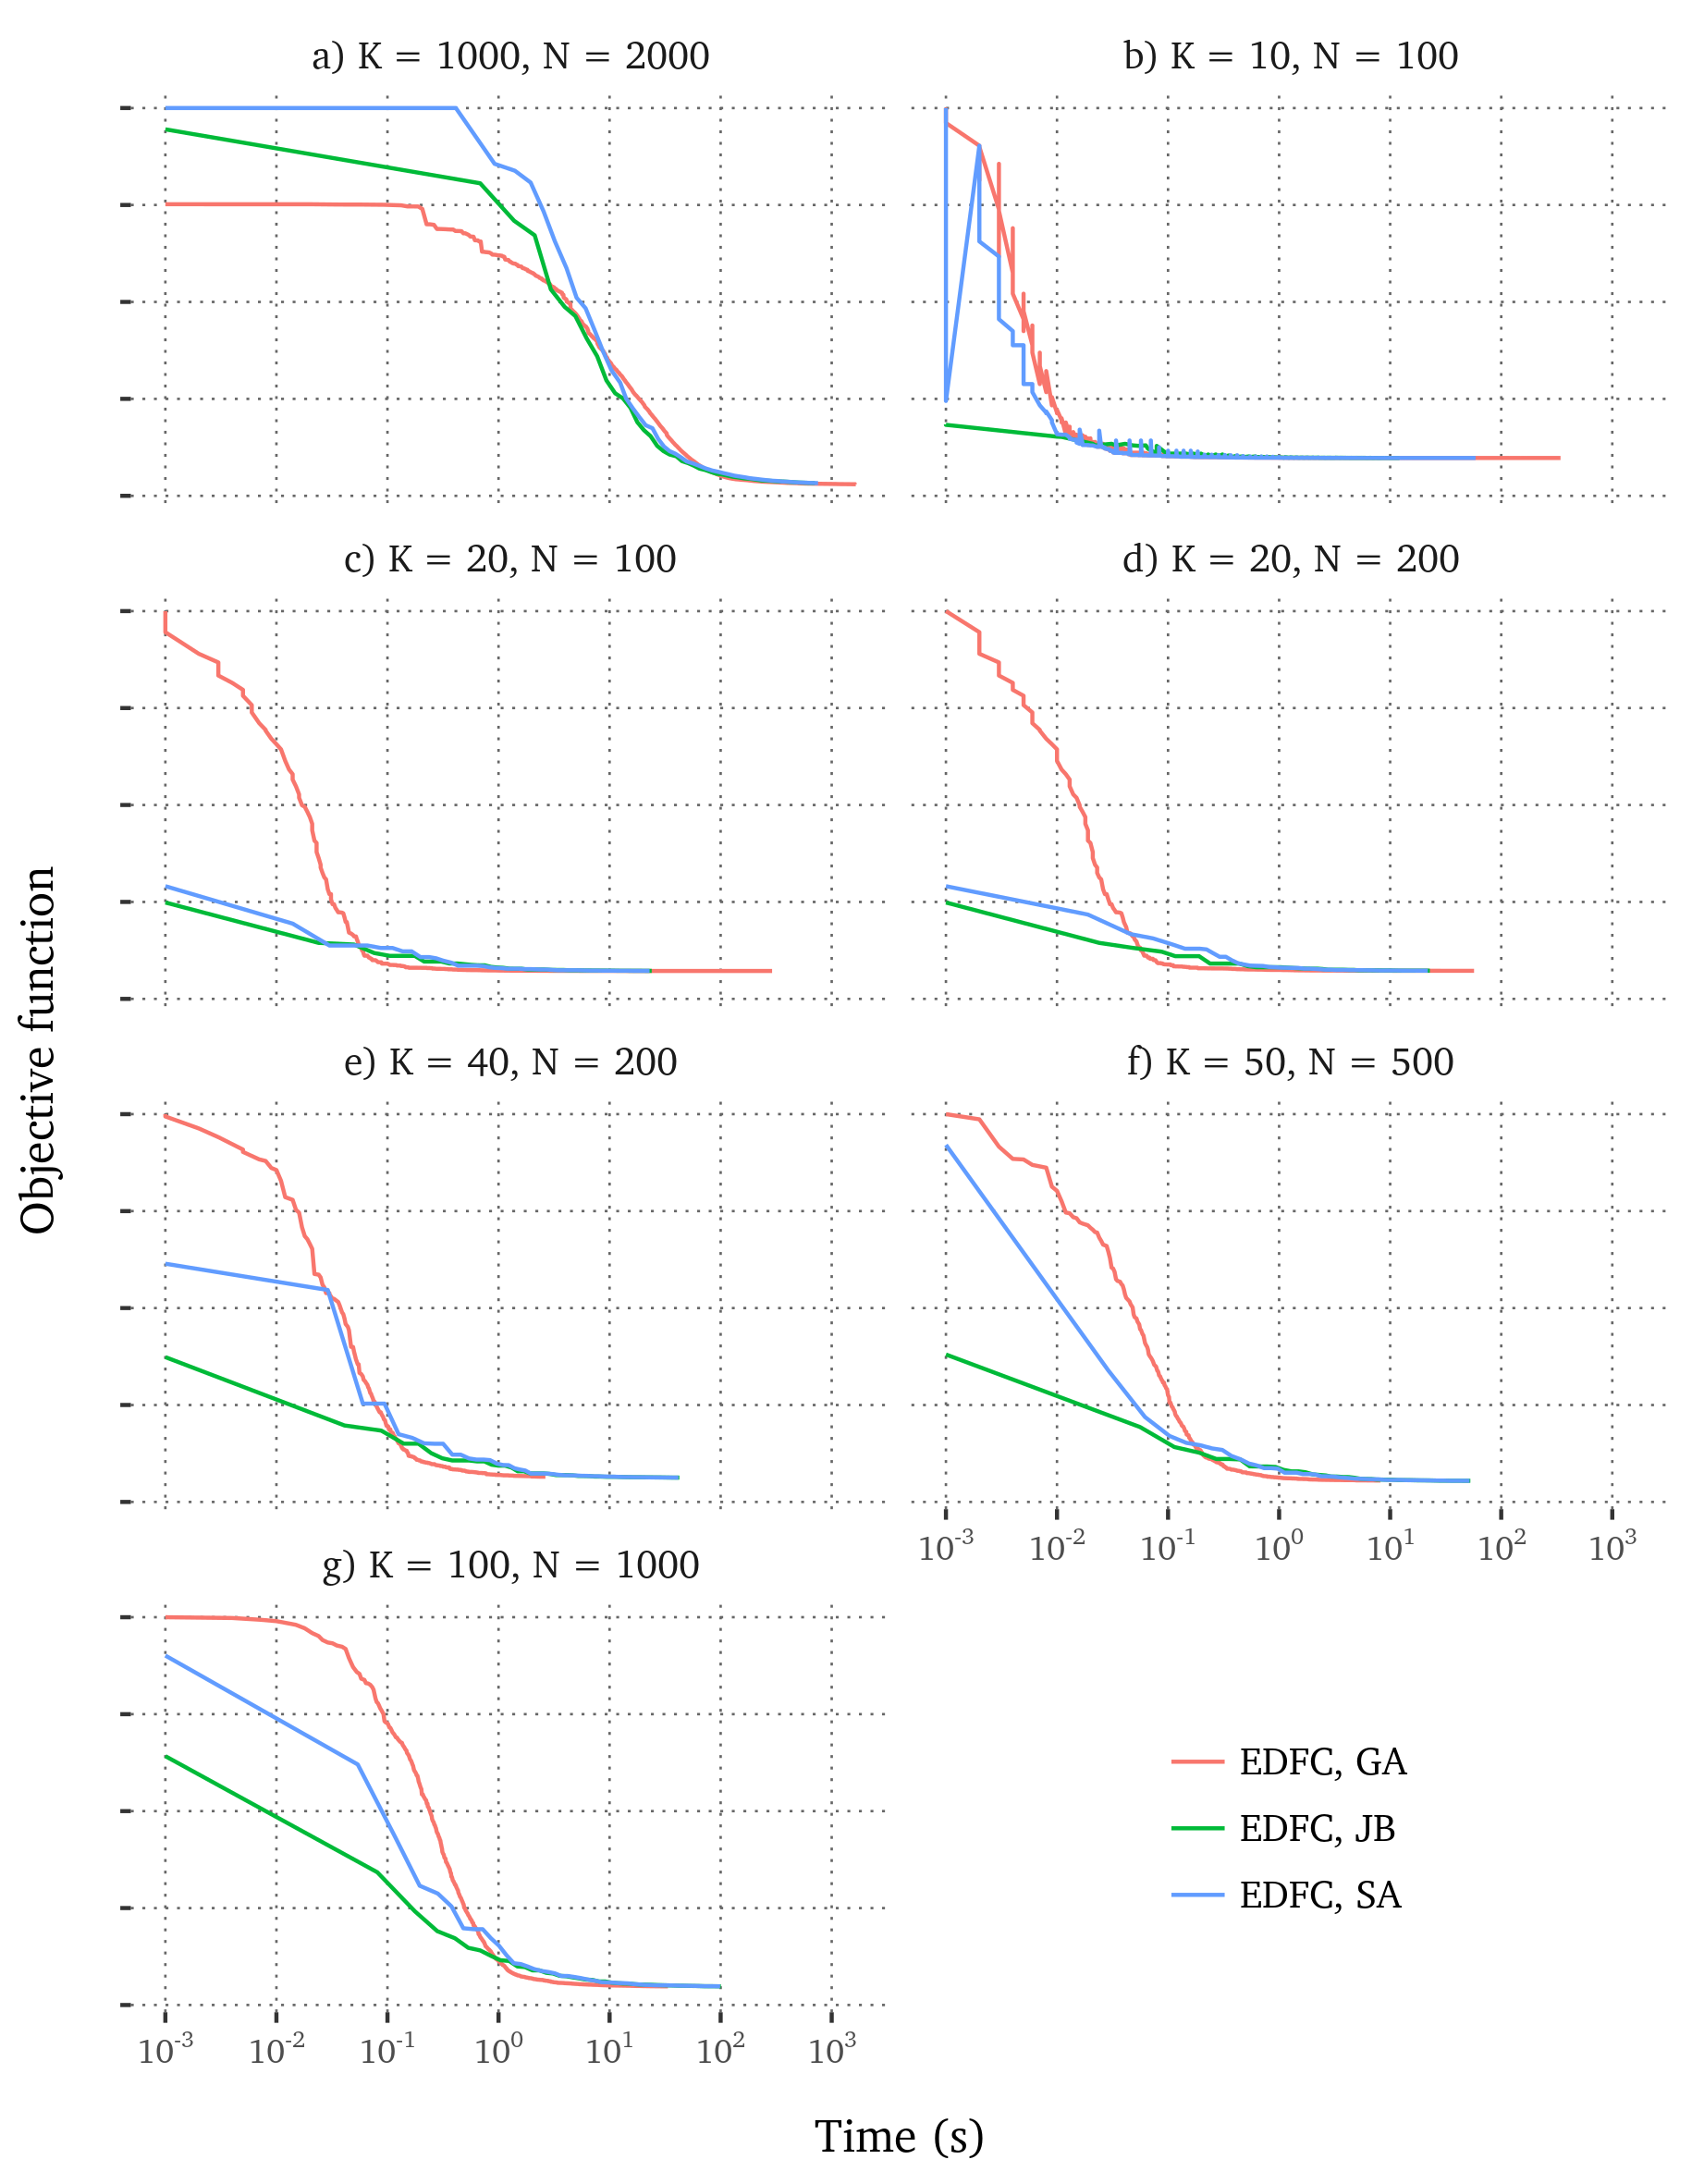
\includegraphics[]{figures/progress-edfc.png}
	\caption{For each configuration in \autoref{tab:results}, normalized ovearhead factor $g_2$ of \gls{adfc} algorithm solutions is plotted against computation time.}
	\label{fig:progress-edfc}
\end{figure}

\begin{figure}[htp]
	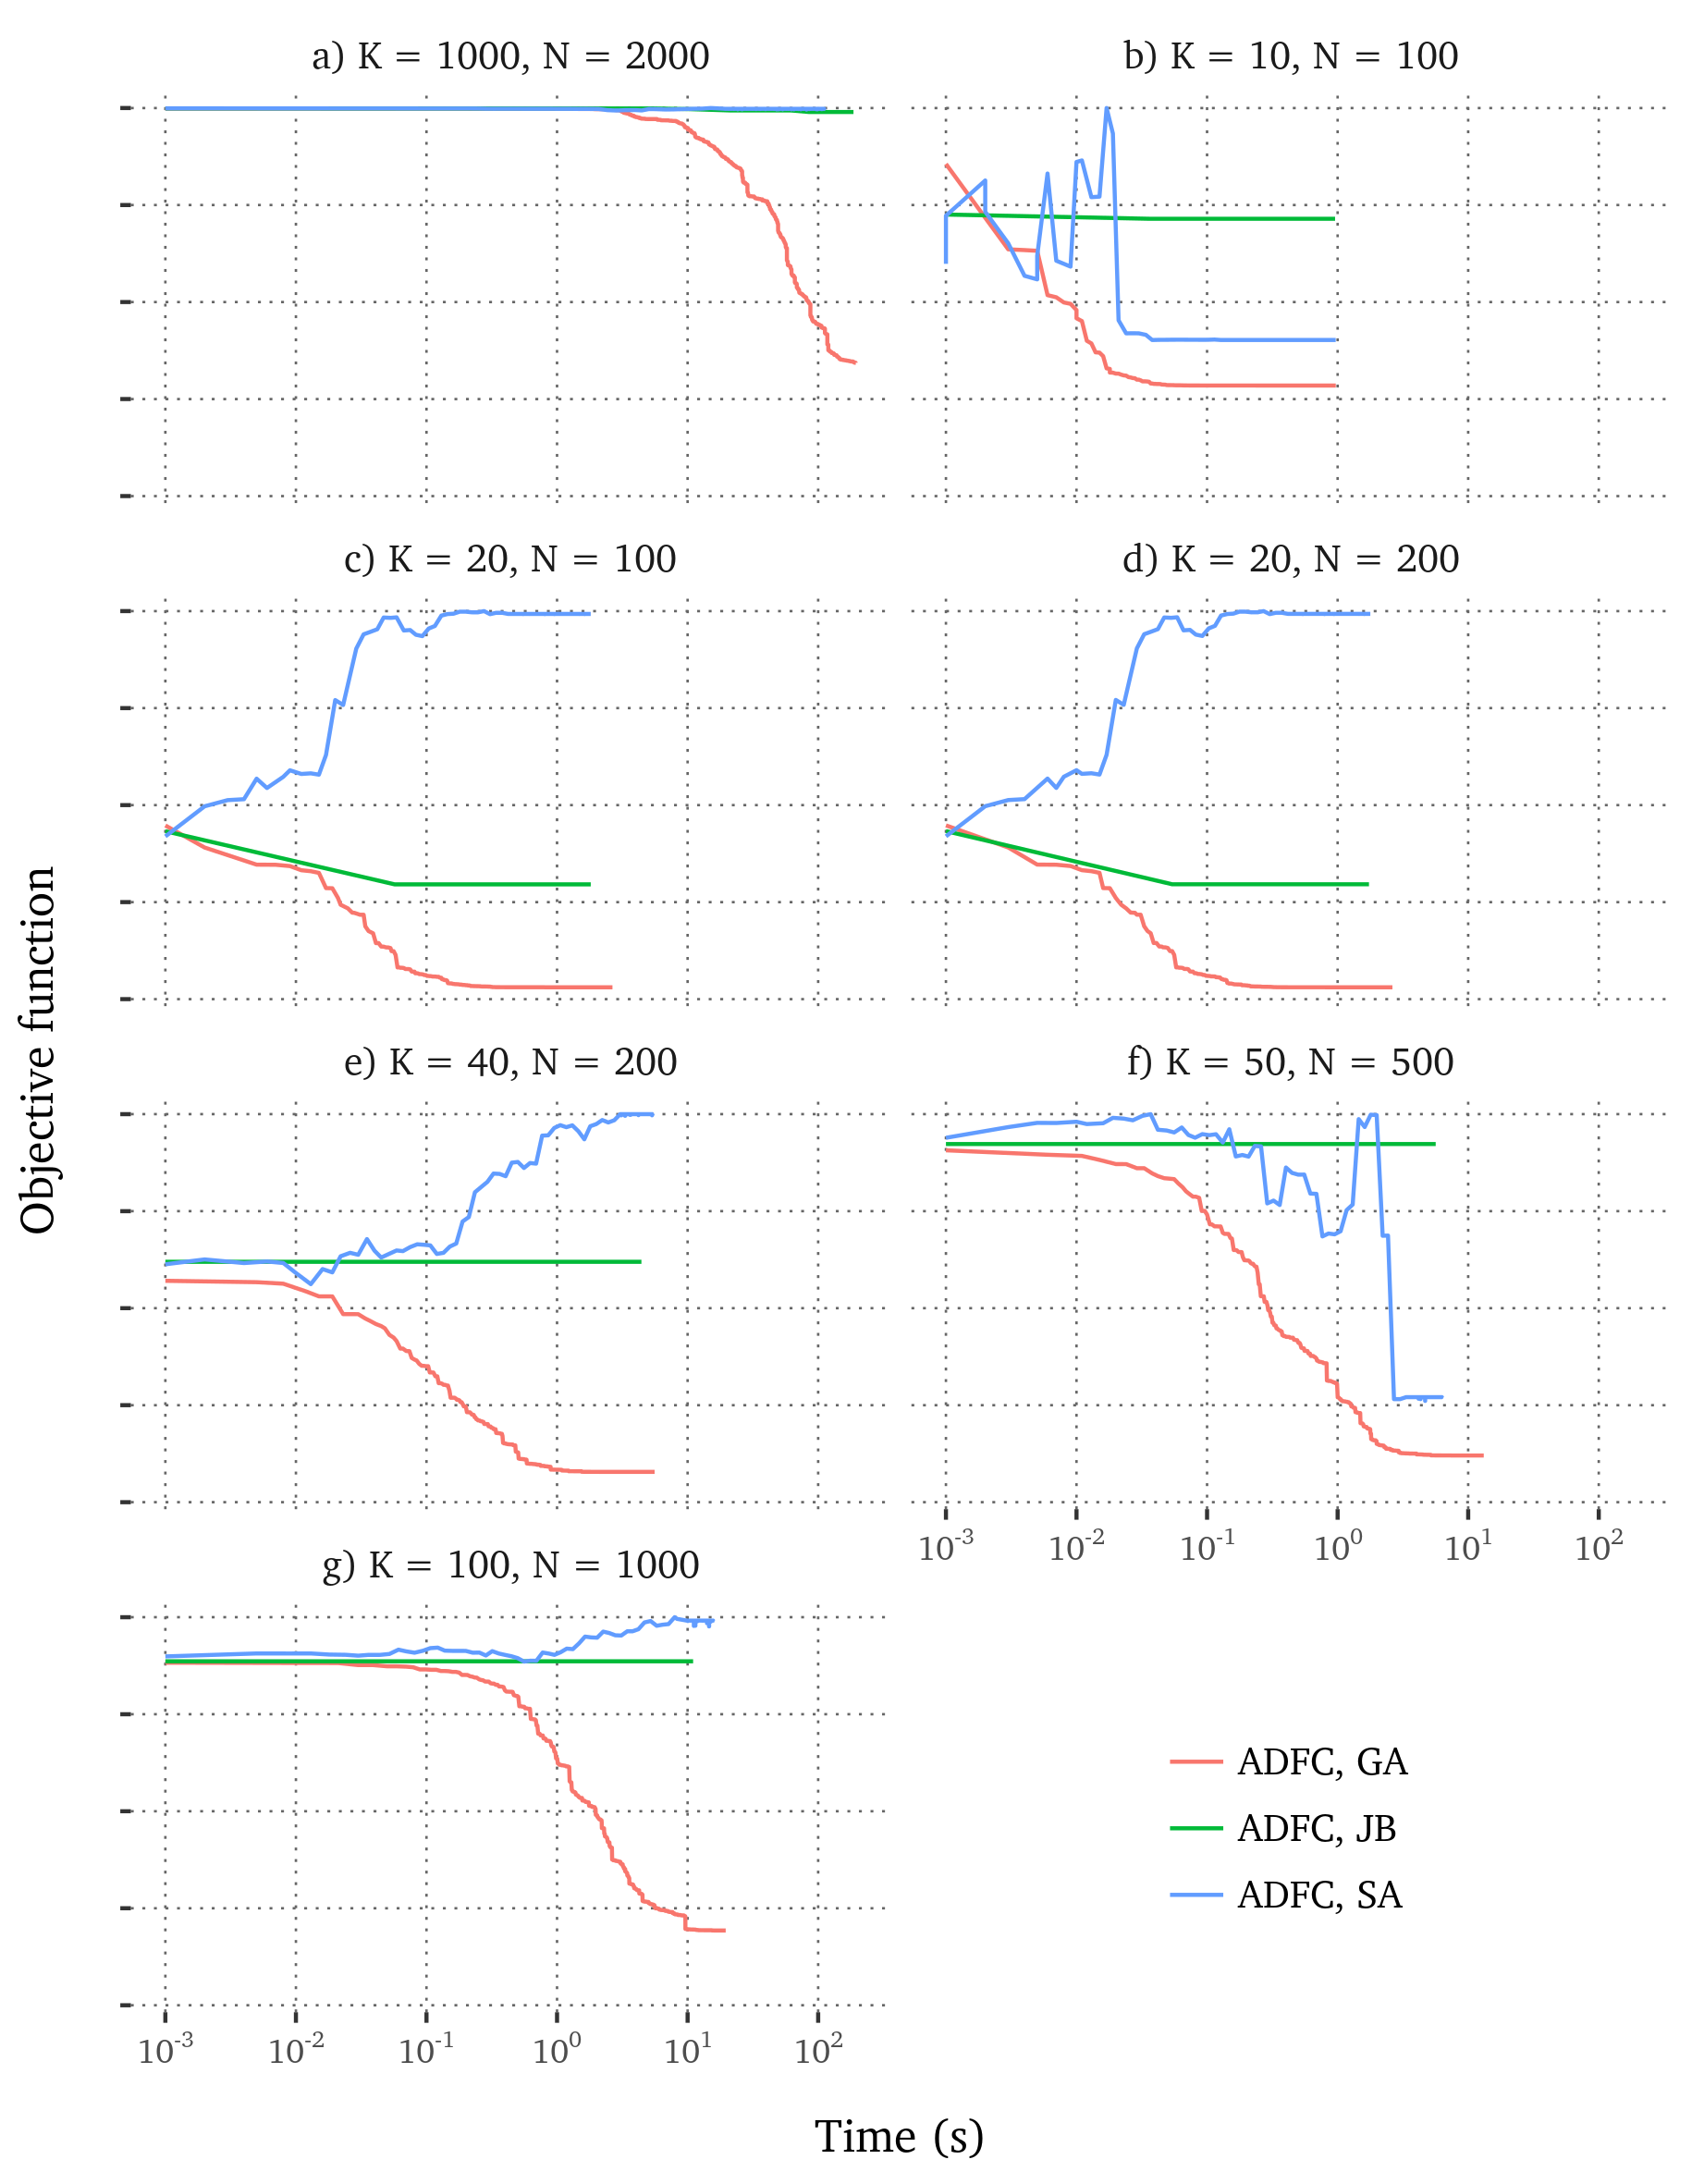
\includegraphics[]{figures/progress-adfc.png}
	\caption{For each configuration in \autoref{tab:results}, normalized score $g_1$ of \gls{edfc} algorithm solutions is plotted against computation time.}
	\label{fig:progress-adfc}
\end{figure}

\begin{figure}[htp]
	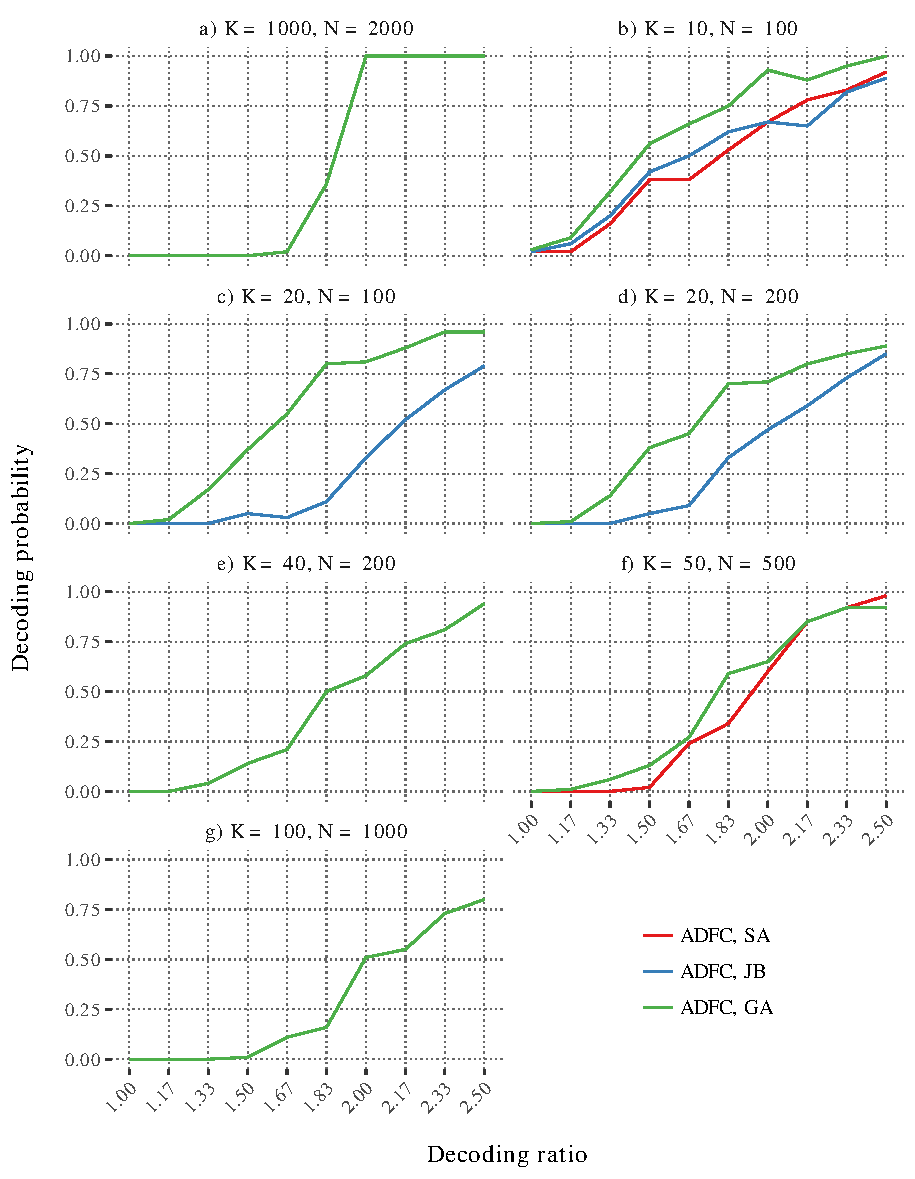
\includegraphics[]{figures/eta_vs_prob_adfc_only.pdf}
	\caption{For each configuration in \autoref{tab:results}, successful deconding probability of \gls{adfc} spreading algorithm has been computed varying decoding ratio $\eta$. Solvers that provided no possibility to packet recovering are here omitted from the plots.}
	\label{fig:eta_vs_prob_adfc_only}
\end{figure}

\begin{figure}[htp]
	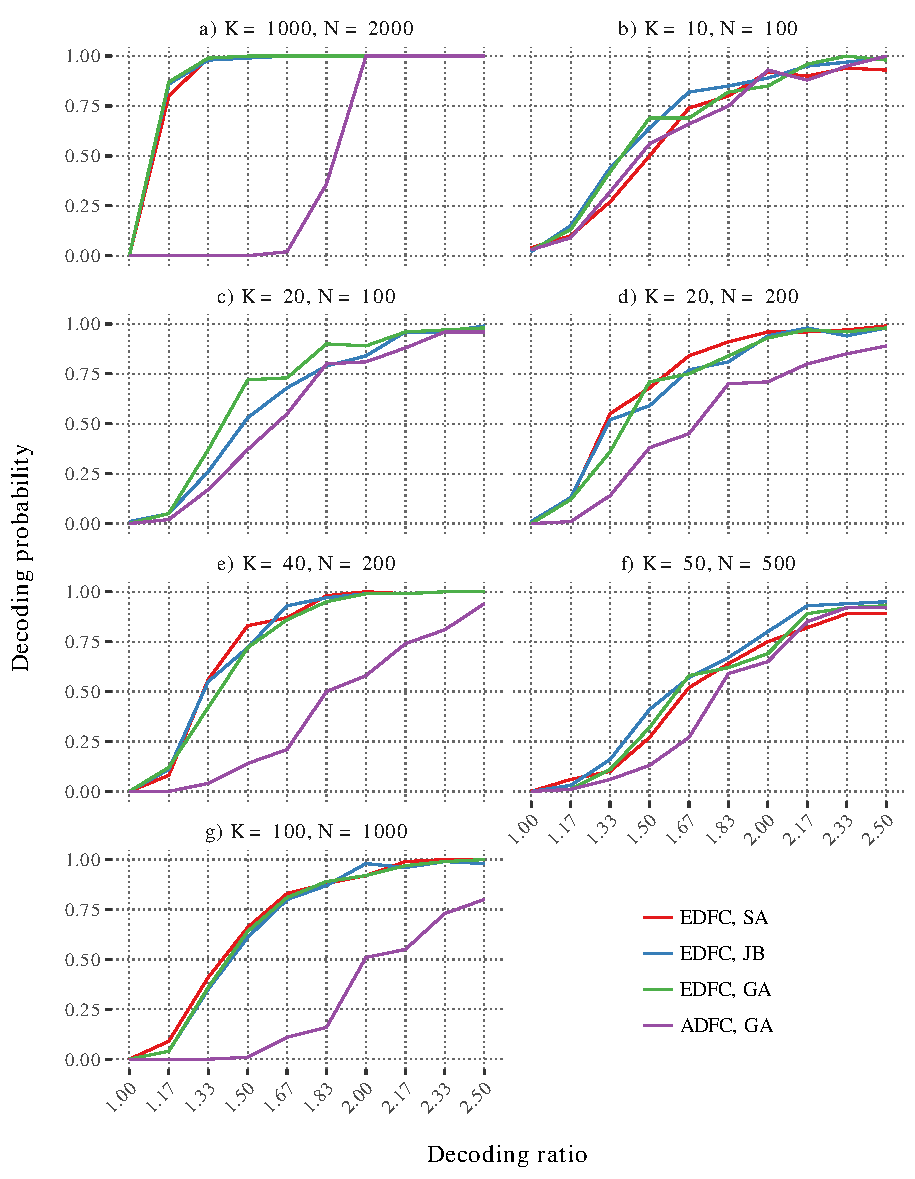
\includegraphics[]{figures/eta_vs_prob_reliable_ones.pdf}
	\caption{For each configuration in \autoref{tab:results}, successful deconding probability of \gls{edfc} and \gls{adfc} (given \gls{ga} solutions) has been computed varying decoding ratio $\eta$.}
	\label{fig:eta_vs_prob_reliable_ones}
\end{figure}

% \glsresetall
\clearpage
\section{Conclusions And Future Work}\label{sec:conclusions}
In this work, we analyze the behaviour of two different spreading algorithms, \gls{adfc} and \gls{edfc}, to perform a network coding in \gls{wsn} as proposed in our reference paper.\cite{Lin2007}

First of all, we solved the two related optimization problems, using well-known algorithms, Genetic Algorithm and Simulated Annealing, and a modified version of the latter, called Jumping Ball.

With the solution provided, we built a network simulator that took into account only the network layer of the ISO-OSI architecture, to generalize our result in various physical and \textsc{MAC} settings.
This simulator was written from scratch by our group in C++ programming language: that made our program much faster than similar tools, such as MATLAB\textregistered.

With our analysis, we confirmed that \gls{adfc} is confirmed to achieve much lower network overhead than \gls{edfc}, in general at the cost of a lower successful decoding probability for small values of $\eta$.
We also stated that heuristic search tecniques are suitable to perform non-convex optimization for \emph{Fountain Code} network conding.
Moreover, we think our results can be improved by the means of other search techniques or perturbation strategies that better fits each problem peculiarities.

\bibliographystyle{IEEEtran}
\bibliography{bibliography}

\end{document}

%%% Local Variables:
%%% mode: latex
%%% TeX-master: t
%%% End:
